\documentclass[aspectratio=169]{beamer}

\usefonttheme[stillsansserifmath]{serif}
\usepackage{graphicx}
\usepackage{amsfonts}
\usepackage{mathtools, nccmath}
\usepackage{amssymb, amsmath}
\usepackage{xspace}
\usepackage{tikz}
\usepackage{standalone}
\usepackage{euler}
\usepackage{color,xcolor}
\usepackage{fontspec}
\usepackage{nameref}
\usepackage{manfnt}
\usepackage{listings}
\usepackage{xcolor}
\usepackage{algorithm}
\usepackage[noend]{algpseudocode}
\usepackage{algorithmicx}
\usepackage{docs/style}

\usepackage{xepersian}
\settextfont{Yas}

% Persian specific
\newcommand{\itmsep}[1]{\raggedleft\setlength\itemsep{#1}}
\newcommand{\itemr}{\raggedleft\setlength\itemsep{3mm}}
\newcommand{\fn}[2]{\LR{\LTRfootnote[frame,#1]{~#2}}}
%\newcommand{\fn}[2]{{\LR{\footnote[frame,#1]{{~\LR{#2}}}}}}
\newcommand{\fnn}[1]{{\LR{\footnote[frame]{{~\LR{#1}}}}}}
\newcommand{\m}[1]{\ensuremath{\mathnormal{#1}}}
\newcommand{\mc}[1]{\ensuremath{\mathtt{#1}}}
\newcommand{\scl}{\ensuremath{\Sigma^*}\xspace}
\newcommand{\gcl}{\ensuremath{\Gamma^*}\xspace}
\newcommand{\gin}{\ensuremath{\mathnormal{\in}}\xspace}
%\newcommand{\gand}{\ensuremath{\mathnormal{\land}}\xspace}
\newcommand{\gand}{\&\&\xspace}
\newcommand{\alglr}{\LTR\ttfamily\small}
\newcommand{\st}[1]{\ensuremath{\mathnormal{\{#1\}}}\xspace}
\newcommand{\gst}[1]{\ensuremath{\mathnormal{\{\text{\texttt{#1}}\}}}\xspace}
\newcommand{\cpp}{C++\xspace}
\newcommand{\enc}[1]{\ensuremath{\mathnormal{\langle#1\rangle}}\xspace}
\newcommand{\abo}[1]{\ensuremath{\mathnormal{O(#1)}}\xspace}
\newcommand{\aso}[1]{\ensuremath{\mathnormal{o(#1)}}\xspace}
\newcommand{\aom}[1]{\ensuremath{\mathnormal{\Omega(#1)}}\xspace}
\newcommand{\ath}[1]{\ensuremath{\mathnormal{\Theta(#1)}}\xspace}
\newcommand{\dom}[2]{\ensuremath{\mathnormal{\Big[ \dfrac{#1}{#2} \Big]}}\xspace}

\newcommand{\Proc}[2]{\Statex \textbf{procedure} \textsc{#1}(#2)}
\newcommand{\Func}[2]{\Statex \textbf{function} \textsc{#1}(#2)}
\newcommand{\To}{\textbf{to}\xspace}
\newcommand{\Aand}{\textbf{and}\xspace}
\newcommand{\Aor}{\textbf{or}\xspace}



\newcommand\pro{\ensuremath{\rightarrow}\xspace}
\newcommand\der{\ensuremath{\Rightarrow}\xspace}
\newcommand\ders{\ensuremath{\stackrel{\mbox{*}}{\Rightarrow}}\xspace}
\newcommand{\dern}[1]{\ensuremath{\stackrel{\mbox{\small #1}}{\Rightarrow}}\xspace}
\newcommand\move{\ensuremath{\vdash}\xspace}
\newcommand\moves{\ensuremath{\stackrel{\small *}{\vdash}}\xspace}
\newcommand{\movesn}[1]{\ensuremath{\stackrel{\small *}{\vdash_{#1}}}\xspace}
\newcommand{\moven}[1]{\ensuremath{\mathnormal{\vdash_{#1}}}\xspace}

\newcommand{\code}[1]{{\LR{\texttt{#1}}}}
\newcommand{\txtlr}[1]{\text{\LR{#1}}}


% Abbreviations
\newcommand{\ie}{\latin{i.e.,~}}
\newcommand{\eg}{\latin{e.g.,~}}
\newcommand{\cf}{\latin{cf.~}}
\newcommand{\etal}{\latin{et al.~}}
\newcommand{\etc}{\unskip~\latin{etc.}\xspace}
\newcommand{\apriori}{\latin{a priori}}
\newcommand{\wrt}{\latin{w.r.t.~}}
%\newtheorem{theorem}{Theorem}

\newcommand\NN{\ensuremath{\mathbb{N}}\xspace}
\newcommand\RR{\ensuremath{\mathbb{R}}\xspace}
\newcommand\NNS{\ensuremath{\mathbb{N}^*}\xspace}
\newcommand\NNZ{\ensuremath{\mathbb{N}\backslash\{0\}}\xspace}
\newcommand\RRP{\ensuremath{\mathbb{R}^+}\xspace}
\newcommand\vect[1]{\ensuremath{\boldsymbol{\vec{#1}}}}
\newcommand\MP{\ensuremath{\mathcal{P}}\xspace}

\newcommand\de{\mathrel{\bullet\mkern-2.5mu{\rightarrow}}}
\newcommand\ue{\mathrel{\bullet\mkern-3mu{-}\mkern-3mu\bullet}}

\DeclareMathOperator*{\argmax}{arg\,max}
\DeclareMathOperator*{\argmin}{arg\,min}

\DeclareMathOperator{\lcm}{lcm}
\DeclareMathOperator{\Spec}{Spec}
\DeclareMathOperator{\Res}{Res}
%\DeclareMathOperator{\land}{and}

\newcommand{\fl}[1]{\ensuremath{\lfloor #1 \rfloor}}
\newcommand{\bfl}[1]{\ensuremath{\big\lfloor #1 \big\rfloor}}
\newcommand{\Bfl}[1]{\ensuremath{\Big\lfloor #1 \Big\rfloor}}
\newcommand{\bgfl}[1]{\ensuremath{\bigg\lfloor #1 \bigg\rfloor}}
\newcommand{\Bgfl}[1]{\ensuremath{\Bigg\lfloor #1 \Bigg\rfloor}}

\newcommand{\cl}[1]{\ensuremath{\lceil #1 \rceil}}
\newcommand{\bcl}[1]{\ensuremath{\big\lceil #1 \big\rceil}}
\newcommand{\Bcl}[1]{\ensuremath{\Big\lceil #1 \Big\rceil}}
\newcommand{\bgcl}[1]{\ensuremath{\bigg\lceil #1 \bigg\rceil}}
\newcommand{\Bgcl}[1]{\ensuremath{\Bigg\lceil #1 \Bigg\rceil}}

\newcommand{\mtx}[1]{\begin{pmatrix} #1 \end{pmatrix}}
\newcommand{\smtx}[1]{\begin{psmallmatrix} #1 \end{psmallmatrix}}

\definecolor{commentgreen}{RGB}{2,112,10}
\definecolor{eminence}{RGB}{108,48,130}
\definecolor{brightmaroon}{rgb}{0.76, 0.13, 0.28}
\definecolor{darkred}{rgb}{0.55, 0.0, 0.0}
\lstset {
    language=C++,
    frame=tb,
    tabsize=4,
    showstringspaces=false,
    numbers=left,
    %upquote=true,
    commentstyle=\color{commentgreen},
    keywordstyle=\color{eminence},
    stringstyle=\color{darkred},
    basicstyle=\small\ttfamily, % basic font setting
    emph={int,char,double,float,unsigned,long,short,void,bool},
    emphstyle={\color{blue}},
    %escapechar=\&,
    % keyword highlighting
    %classoffset=1, % starting new class
    %otherkeywords={>,<,.,;,-,!,=,~},
    %morekeywords={>,<,.,;,-,!,=,~},
    %keywordstyle=\color{weborange},
    %classoffset=0,
}

\makeatletter
\NewDocumentCommand{\LeftComment}{s m}{%
	\IfBooleanF{#1}{\hspace*{\ALG@thistlm}}\textcolor{commentgreen}{\(~\triangleright\) #2}}
\makeatother


\newenvironment{itemframe}[2]{
\begin{frame}[environment=itemframe]{#1}

\framesubtitle{\small \color{gray} \quad #2}
\itemize
\itemr

}{
\enditemize
\end{frame}
}

\newcommand{\centerimg}[2][.5]{
    \begin{figure}[h!]
        \centering
        \includegraphics[width=#1\textwidth]{#2}
    \end{figure}
}

\usetikzlibrary{arrows,calc}
\usetikzlibrary{positioning,shapes,chains,fit}


\tikzset{
    %Define style for boxes
    node/.style={
        circle,
        draw=black, thick,
        align=center,
    },
    ss/.style={
        circle,
        draw=black,
        align=center,
    },
    proc/.style={
        rounded corners,
        draw=black,
        align=center,
    },
    ifelse/.style={
	ellipse,
	draw=black,
	align=center,
    },
    cloudy/.style={
	cloud,
	cloud puffs=12,
	cloud ignores aspect,
	align=center,
	draw=black,
    },
    txt/.style={
        draw = none,
        align = center,
        font = \footnotesize,
    },
    coin/.style={
        rectangle,
        minimum height=1mm,
        minimum width=1cm,
        draw=black,
        fill=black!20,
        rounded corners
    },
    towercolor/.style={
        fill=black!80
    },
    towerbase/.style={
        trapezium,
        trapezium angle=75,
        trapezium stretches=true,
        towercolor,
        minimum width=7mm,
        minimum height=2mm,
    },
    tower/.style={
        rectangle,
        rounded corners,
        towercolor,
        minimum width=2mm,
        minimum height=26mm,
    },
    start-end/.style={
        draw,
        rectangle,
        rounded corners,
    },
    input/.style={ % requires library shapes.geometric
        draw,
        trapezium,
        trapezium left angle=60,
        trapezium right angle=120,
    },
    operation/.style={
        draw,
        rectangle
    },
    loop/.style={ % requires library shapes.misc
        draw,
        chamfered rectangle,
        chamfered rectangle xsep=2cm
    },
    decision/.style={ % requires library shapes.geometric
        draw,
        diamond,
        aspect=#1
    },
    decision/.default=1,
    print/.style={ % requires library shapes.symbols
        draw,
        tape,
        tape bend top=none
    },
    connection/.style={
        draw,
        circle,
        radius=5pt,
    },
    process rectangle outer width/.initial=0.15cm,
    predefined process/.style={
        rectangle,
        draw,
        append after command={
        \pgfextra{
          \draw
          ($(\tikzlastnode.north west)-(0,0.5\pgflinewidth)$)--
          ($(\tikzlastnode.north west)-(\pgfkeysvalueof{/tikz/process rectangle outer width},0.5\pgflinewidth)$)--
          ($(\tikzlastnode.south west)+(-\pgfkeysvalueof{/tikz/process rectangle outer width},+0.5\pgflinewidth)$)--
          ($(\tikzlastnode.south west)+(0,0.5\pgflinewidth)$);
          \draw
          ($(\tikzlastnode.north east)-(0,0.5\pgflinewidth)$)--
          ($(\tikzlastnode.north east)+(\pgfkeysvalueof{/tikz/process rectangle outer width},-0.5\pgflinewidth)$)--
          ($(\tikzlastnode.south east)+(\pgfkeysvalueof{/tikz/process rectangle outer width},0.5\pgflinewidth)$)--
          ($(\tikzlastnode.south east)+(0,0.5\pgflinewidth)$);
        }  
        },
        text width=#1,
        align=center
    },
    predefined process/.default=1.75cm,
    man op/.style={ % requires library shapes.geometric
        draw,
        trapezium,
        shape border rotate=180,
        text width=2cm,
        align=center,
    },
    extract/.style={
        draw,
        isosceles triangle,
        isosceles triangle apex angle=60,
        shape border rotate=90
    },
    merge/.style={
        draw,
        isosceles triangle,
        isosceles triangle apex angle=60,
        shape border rotate=-90
    },
}


\title{طراحی الگوریتم‌ها}
\author{
آرش شفیعی
}

\institute{
\\

\includegraphics[height=1.2cm]{logos/ui.png}
%\\
%دانشگاه اصفهان
}
\date{}

\begin{document}

\begin{frame}[plain]
\begin{center}
به نام خدا
\end{center}

\maketitle

%\begin{center}
%{\footnotesize arash.shafiei@gmail.com}
%\end{center}

\end{frame}
\setcounter{framenumber}{0}

%\input{docs/licence}

\raggedleft

%%%%%%%%%%%%
%\begin{frame}{فهرست مطالب}
%\begin{flushright}
%  \tableofcontents
%\end{flushright}
%\end{frame}
%%%%%%%%%%%%

%%%%%%%%%%%%
%%%%%%%%%%%%%%%%%%%%%%%%%
\section{جستجوی ترکیبیاتی}
%%%%%%%%%%%%%%%%%%%%%%%%%

\begin{frame}{‌جستجوی ترکیبیاتی}
\begin{itemize}\itemr
\item[-]
روش‌های تقسیم و حل، برنامه‌ریزی پویا و حریصانه را برای حل دسته‌ای از مسئله‌های محاسباتی بررسی کردیم. در مسئله‌های بررسی شده، یک راه‌حل ساده برای پیدا کردن جواب مسئله جستجوی همهٔ حالت‌ها است ولی چنین جستجویی در زمان معقول (زمان چند جمله‌ای) امکان پذیر نیست چرا که تعداد همهٔ حالت‌های ممکن از مرتبه نمایی است و بنابراین جستجوی همهٔ حالت‌ها در زمان نمایی صورت می‌گیرد. توسط روش‌های تقسیم و حل، برنامه‌ریزی پویا و حریصانه روش‌هایی برای حل مسئله‌ها در زمان معقول ارائه کردیم.
\item[-]
پیدا کردن جواب در زمان چند جمله‌ای برای همهٔ مسئله‌ها همیشه امکان پذیر نیست و گاهی تنها راه حل ، جستجوی فضای حالت برای آن مسئله است. جستجوی فضای حالت به معنی تولید همهٔ جواب‌های مسئله و انتخاب حالت بهینه یا حالت مورد نظر از بین همهٔ حالت‌های ممکن است. تعداد این حالت‌ها از مرتبهٔ نمایی است و بنابراین چنین الگوریتم‌هایی به زمان نمایی برای محاسبه نیاز دارند و در نتیجه برای مسائلی با اندازهٔ بزرگ در عمل قابل استفاده نیستند.
\end{itemize}
\end{frame}


\begin{frame}{‌جستجوی ترکیبیاتی}
\begin{itemize}\itemr
\item[-]
در مبحث جستجوی ترکیبیاتی
\fn{1}{combinatorial search}
، روش‌های جستجوی همه فضای حالت برای یک مسئله بررسی می‌شود. در این روش‌ها مطالعه می‌کنیم چگونه به طور منظم همهٔ حالت‌ها را بررسی کنیم و یا اینکه چگونه با استفاده از روش‌هایی فضای حالت را محدود کنیم.
\item[-]
ترکیبیات
\fn{2}{combinatorics}
شاخه‌ای از ریاضیات است که در آن به بررسی ساختارهای متناهی و شمارش این ساختارها می‌پردازیم.
\item[-]
برای مثال گراف یک ساختار متناهی است و تعداد مسیرها در یک گراف، متناهی است. برای پیدا کردن بلندترین مسیر در یک گراف می‌توانیم همهٔ مسیرها را بررسی و بلندترین آنها را انتخاب کنیم.
\item[-]
بهینه سازی ترکیبیاتی
\fn{3}{combinatorial optimization}
شاخه‌ای از بهینه‌سازی است که در آن مجموعهٔ جواب‌های امکان پذیر گسسته است و هدف پیدا کردن جواب بهینه از بین همهٔ جواب‌های ممکن است.
\end{itemize}
\end{frame}

\begin{frame}{‌پسگرد}
\begin{itemize}\itemr
\item[-]
روش پسگرد
\fn{1}{backtrack}
روشی است که با استفاده از آن همهٔ فضای حالت را جستجو می‌کنیم. در این روش با یکی از حالت‌ها در فضای حالت شروع می‌کنیم و برای انتخاب حالت بعد یکی از پارامترهای فضای حالت را تغییر می‌دهیم. ممکن است در انتخاب حالت بعد، چند پارامتر قابل تغییر باشند. در اینصورت یکی از پارامترها را تغییر می‌دهیم و به حالت بعد می‌رویم و سپس پسگرد می‌کنیم تا یکی دیگر از پارامترها را تغییر دهیم. بدین صورت همهٔ حالت‌ها در فضای حالت بررسی می‌شوند.
\end{itemize}
\end{frame}

\iffalse
\begin{frame}{‌پسگرد}
\begin{itemize}\itemr
\item[-]
برای مثال فرض کنید می‌خواهیم همهٔ رشته‌ها با طول ۲ که از سه حرف a و b و c تشکیل شده‌اند را بشماریم. یا به عبارت دیگر همهٔ فضای حالت را تولید کنیم.
\item[-]
با استفاده از روش پسگرد در ابتدا ۳ انتخاب برای حرف اول داریم حرف a را انتخاب می‌کنیم و سپس از بین ۳ انتخاب برای حرف دوم، حرف a را انتخاب می‌کنیم پس رشتهٔ aa را به دست می‌آوریم، سپس پسگرد می‌کنیم و حرف b را برای حرف دوم رشته انتخاب می‌کنیم و رشته ab را بدست می‌آوریم. بار دیگر با یک پسگرد رشتهٔ ac را بدست می‌آوریم. در پسگرد بعدی هیچ انتخابی برای حرف دوم وجود نخواهد داشت پس دوباره پسگرد می‌کنیم و حرف b را به عنوان حرف اول انتخاب می‌کنیم. با استفاده از این روش به ترتیب رشته‌های
ba
،
bb
،
bc
،
ca
،
cb
و
cc
به دست می‌آیند.
\end{itemize}
\end{frame}
\fi

\begin{frame}{‌پسگرد}
\begin{itemize}\itemr
\item[-]
فرض کنید وارد یک باغ پر پیچ و خم یا باغ هزارتو
\fn{1}{maze}
شده‌اید و می‌خواهید راه خروجی را پیدا کند. راه را در پیش می‌گیرید و به هر چند راهی که می‌رسید راه اول از سمت چپ را انتخاب می‌کنید. در پایان یا راه خروجی را پیدا می‌کنید و یا به بن‌بست بر می‌خورید. در صورتی که به بن‌بست رسیدید، بازمی‌گردید تا به اولین چندراهی قبل از بن‌بست برسید. به جای راه اول از سمت چپ، دومین راه از سمت چپ را امتحان می‌کنید و در صورت برخورد با بن‌بست راه را باز می‌گردید و در چند راهی راه سوم را امتحان می‌کنید. فرض کنید که همهٔ راه‌ها در چند راهی آخر را امتحان کردید و به بن‌بست خوردید. در این صورت باید مسیر را بازگردید تا به دومین چند راهی قبل از بن‌بست برسید و این بار در دومین چندراهی قبل از بن‌بست، دومین راه را انتخاب کنید. این روند را ادامه می‌دهید تا راه خروجی را پیدا کنید. به این روش حل مسئله روش پسگرد گفته می‌شود.
\item[-]
هر یک از چندراهی‌ها یکی از پارامترهای مسئله است که مقادیر مختلف آن را امتحان می‌کنید.
\end{itemize}
\end{frame}


\begin{frame}{‌پسگرد}
\begin{itemize}\itemr
\item[-]
روش پسگرد وقتی استفاده می‌شود که می‌خواهیم مسئله‌ای را حل کنیم که در آن عناصر یک دنباله
\fn{1}{sequence}
باید از اشیائی از یک مجموعهٔ
\fn{2}{set}
معین انتخاب شوند، به طوری‌که دنباله ویژگی مشخصی داشته باشد و معیار
\fn{3}{criterion}
معینی را برآورده کند.
\end{itemize}
\end{frame}

\begin{frame}{مسئلهٔ چند وزیر}
\begin{itemize}\itemr
\item[-]
می‌خواهیم تعداد n وزیر را در یک صفحه شطرنج
\m{n \times n}
به گونه‌ای قرار دهیم که هیچ یک از وزیرها همدیگر را تهدید نکنند. به عبارت دیگر هیچ دو وزیری نباید در یک سطر یا ستون یا خط مورب مشترکی قرار بگیرند.
\item[-]
دنباله‌ای که در این مسئله به دنبال آن می‌گردیم، دنباله‌ای است از n مکان که n وزیر در آنها قرار گرفته‌اند. مجموعه‌ای که هر یک از عناصر دنباله می‌توانند از  اعضای آن مجموعه انتخاب شوند عبارت است از مجموعه‌ای شامل
\m{n^2}
مکان بر روی صفحهٔ شطرنج.
\item[-]
ویژگی معینی که این دنباله باید داشته باشد این است که هیچ دو مکان انتخاب شده‌ای بر روی یک خط افقی، عمودی یا مورب قرار نگیرد.
\item[-]
مسئلهٔ چند وزیر یا
n
وزیر،
 حالت کلی مسئلهٔ ۸ وزیر است که در آن ۸ وزیر در یک صفحه شطرنج استاندارد با تعداد
۸ $\times$ ۸
مکان قرار می‌گیرند.
\item[-]
در اینجا برای سهولت نمایش حالات مختلف مسئله ۴ وزیر را در نظر می‌گیریم.
\end{itemize}
\end{frame}


\begin{frame}{مسئلهٔ چند وزیر}
\begin{itemize}\itemr
\item[-]
روش پسگرد در واقع روشی است که در یک درخت
\fn{1}{tree}
به صورت عمق-اول
\fn{2}{depth-first}
جستجو می‌کند. پس ابتدا جستجوی عمق-اول در درخت را توضیح می‌دهیم.
\item[-]
فرض کنید درختی داریم که از تعدادی رأس و یال تشکیل شده است و می‌خواهیم همهٔ مسیرهای درخت را که با ریشه شروع می‌شوند و با یک برگ پایان می‌یابند بررسی کنیم.
\item[-]
در واقع دنباله‌هایی که در اینجا بررسی می‌کنیم دنباله‌هایی هستند که یک مسیر در درخت را نشان می‌دهند و با ریشه آغاز و با یکی از برگ‌ها پایان می‌یابند.
\end{itemize}
\end{frame}


\begin{frame}{مسئلهٔ چند وزیر}
\begin{itemize}\itemr
\item[-]
ابتدا به سراغ ریشهٔ درخت می‌رویم و ریشه را به عنوان اولین عنصر دنباله انتخاب می‌کنیم. سپس اولین فرزند از سمت چپ در سطح یک درخت را انتخاب می‌کنیم و اگر این رأس دارای فرزند بود اولین فرزند آن را در سطح دو انتخاب می‌کنیم. این کار را ادامه می‌دهیم تا به یک برگ برسیم. تا اینجا یک مسیر در درخت را بررسی کرده‌ایم. با فرض اینکه برگ در سطح n قرار دارد، به رأس پدر در سطح
\m{n-1}
باز می‌گردیم و فرزند دوم را انتخاب می‌کنیم. این کار را ادامه می‌دهیم تا مسیر دوم و به همین ترتیب همهٔ مسیرها در درخت را بررسی کنیم.
\end{itemize}
\end{frame}


\begin{frame}{مسئلهٔ چند وزیر}
\begin{itemize}\itemr
\item[-]
درخت زیر را در نظر بگیرید. با استفاده از روش پسگرد ابتدا مسیر
\m{(1,2,3)}
سپس
\m{(1,2,4,5)}
سپس
\m{(1,2,4,6)}
، و به همین ترتیب
\m{(1,2,7)}
،
\m{(1,8,9)}
،
\m{(1,8,10)}
، الی آخر بررسی می‌شوند.
\begin{figure}
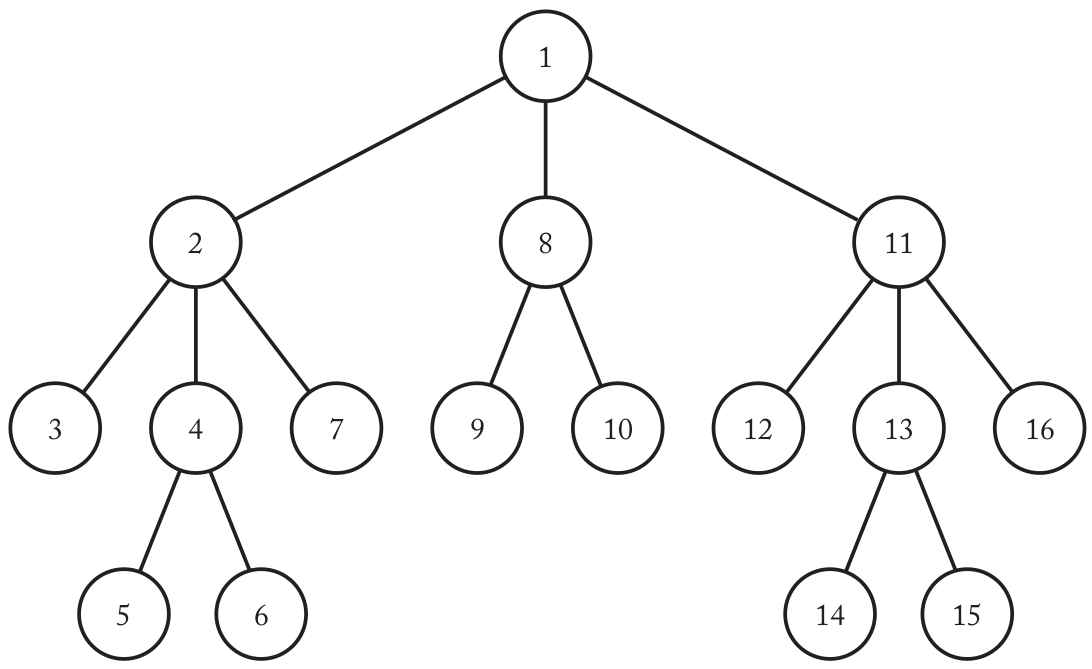
\includegraphics[width=0.6\textwidth]{figs/chap06/tree-backtrack}
\end{figure}
\end{itemize}
\end{frame}


\begin{frame}{مسئلهٔ چند وزیر}
\begin{itemize}\itemr
\item[-]
الگوریتم زیر این روش پسگرد را نشان می‌دهد.
\begin{algorithm}[H]\alglr
  \caption{Depth First TreeSearch} 
  \begin{algorithmic}[1]
   \Func{Depth-First-Tree-Search}{node v}
	 \State visit(v)
	 \For{each child u of v}
   			\State Depth-First-Tree-Search(u)
   	 \EndFor                     
  \end{algorithmic}
  \label{alg:merge}
\end{algorithm}
\end{itemize}
\end{frame}


\begin{frame}{مسئلهٔ چند وزیر}
\begin{itemize}\itemr
\item[-]
حال که با روش پسگرد آشنا شدیم، مسئلهٔ ۴ وزیر را در نظر می‌گیریم. می‌خواهیم ۴ وزیر را در یک صفحهٔ شطرنج
۴ $\times$ ۴
به گونه‌ای قرار دهیم که هیچ دو وزیری یکدیگر را تهدید نکنند. از آنجایی که هیچ دو وزیری نمی‌توانند در یک سطر قرار بگیرند، پس هر وزیر را باید در یک سطر متفاوت از بقیه وزیرها قرار دهیم. از آنجایی که هر وزیر در هر یک از ستون‌ها می تواند قرار بگیرد، بنابراین تعداد همهٔ حالت‌هایی که باید بررسی شوند برابر است با
۲۵۶ = ۴ $\times$ ۴ $\times$ ۴ $\times$ ۴.
\item[-]
برای بررسی همهٔ حالت‌ها درختی تشکیل می‌دهیم که در آن،
مکان اولین وزیر در سطح یک انتخاب می‌شود و مکان وزیر دوم در سطح دوم و به همین ترتیب مکان وزیر سوم در سطح سوم و مکان وزیر چهارم در سطح چهارم انتخاب می‌شوند.
\item[-]
یک مسیر از ریشه تا برگ درواقع یکی از گزینه‌های انتخاب مکان‌های صفحه را نشان می‌دهد. یک گزینه جواب مسئله است اگر در آن هیچ دو وزیری یکدیگر را تهدید نکنند.
\item[-]
به درخت تشکیل شده درخت فضای حالت گفته می‌شود.
\end{itemize}
\end{frame}


\begin{frame}{مسئلهٔ چند وزیر}
\begin{itemize}\itemr
\item[-]
قسمتی از درخت فضای حالات مسئله ۴ وزیر در شکل زیر نمایش داده شده است.
\begin{figure}
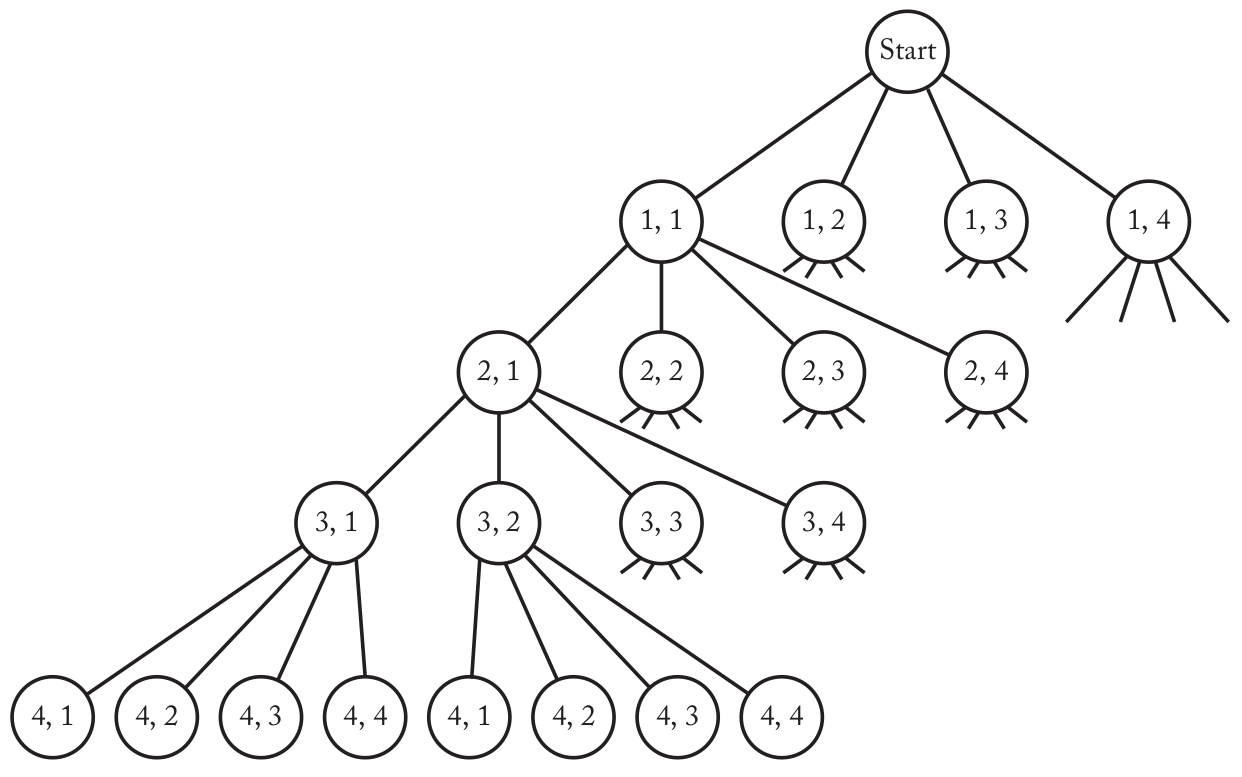
\includegraphics[width=0.7\textwidth]{figs/chap06/n-queens-tree}
\end{figure}
\end{itemize}
\end{frame}


\begin{frame}{مسئلهٔ چند وزیر}
\begin{itemize}\itemr
\item[-]
این درخت در مجموع ۲۵۶ برگ دارد که هر مسیر از ریشه تا یکی از برگ‌ها یکی از گزینه‌ها را نشان می‌دهد. در هریک از رأس‌های درخت یک جفت
\m{(i,j)}
ذخیره می‌شود که برابر با یک مکان در صفحهٔ شطرنج در سطر i و ستون j است.
\end{itemize}
\end{frame}


\begin{frame}{مسئلهٔ چند وزیر}
\begin{itemize}\itemr
\item[-]
 جستجو در این درخت می تواند بهینه‌تر از بررسی همهٔ ۲۵۶ انتخاب نیز انجام شود. برای مثال وقتی وزیر اول در مکان
\m{(1,1)}
قرار گرفت، بدیهی است که وزیر دوم نمی‌تواند در مکان
\m{(2,1)}
قرار بگیرد پس این مسیر در درخت ادامه داده نمی‌شود. همینطور وزیر دوم نمی‌تواند در مکان دوم قرار بگیرد پس نیازی نداریم این مسیر را نیز ادامه دهیم.
\item[-]
در شکل زیر این بهینه‌سازی نشان داده شده است.
\begin{figure}
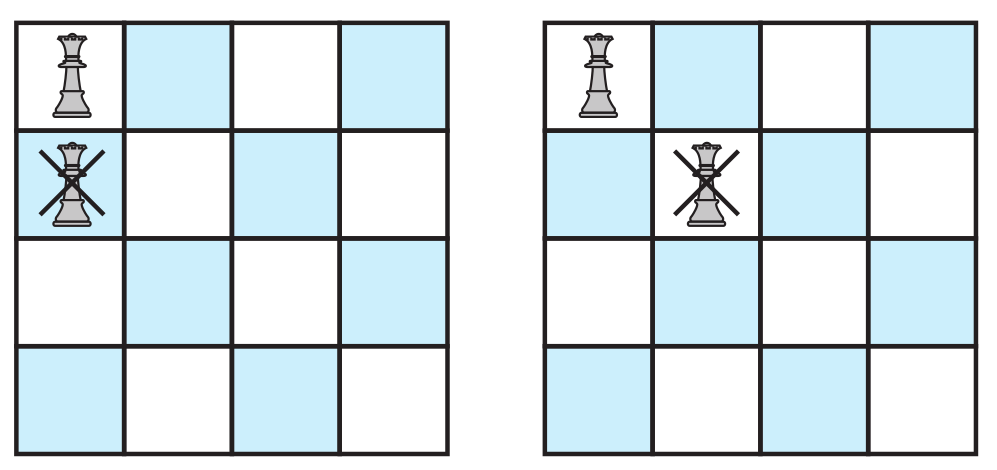
\includegraphics[width=0.6\textwidth]{figs/chap06/n-queens-opt}
\end{figure}
\end{itemize}
\end{frame}


\begin{frame}{مسئلهٔ چند وزیر}
\begin{itemize}\itemr
\item[-]
پسگرد عبارت است از روندی که توسط آن وقتی در یک انتخاب به یک گزینهٔ غیر جواب می‌رسیم، در درخت فضای حالت به عقب بازمی‌گردیم یا به عبارت دیگر از انتخاب یک رأس صرف نظر می‌کنیم و به رأس پدر پسگرد می‌کنیم تا فرزند بعدی پدر را انتخاب کنیم.
\item[-]
به یک رأس در درخت فضای حالت نومید کننده
\fn{1}{nonpromising}
می‌گوییم، اگر انتخاب آن رأس به جواب نیانجامد و به همین ترتیب به یک رأس امید دهنده
\fn{2}{promising}
می‌گوییم اگر با انتخاب آن همچنان احتمال رسیدن به جواب وجود داشته باشد.
\end{itemize}
\end{frame}


\begin{frame}{مسئلهٔ چند وزیر}
\begin{itemize}\itemr
\item[-]
به طور خلاصه در روش پسگرد، بر روی درخت فضای حالت، جستجوی عمق اول انجام می‌دهیم و در فرایند جستجو اگر به رأس نومید کننده برخورد کردیم مسیر را ادامه نمی‌دهیم و به رأس پدر پسگرد می‌کنیم.
\item[-]
به این روش هرس‌کردن
\fn{1}{pruning}
فضای حالت نیز گفته می‌شود که در آن تعدادی از دنباله‌ها بررسی نمی‌شوند.
\end{itemize}
\end{frame}


\begin{frame}{مسئلهٔ چند وزیر}
\begin{itemize}\itemr
\item[-]
در حالت کلی این الگوریتم به صورت زیر نوشته می‌شود.
\begin{algorithm}[H]\alglr
  \caption{Checknode} 
  \begin{algorithmic}[1]
   \Func{Checknode}{node v}
   \If{promising(v)}
   		\If{there is a solution at v}
   				\State write the solution
   		\Else
   			\For{each child u of v}
   					\State Checknode(u)
   			\EndFor
   		\EndIf
   	\EndIf                           
  \end{algorithmic}
  \label{alg:merge}
\end{algorithm}
\end{itemize}
\end{frame}


\begin{frame}{مسئلهٔ چند وزیر}
\begin{itemize}\itemr
\item[-]
ریشهٔ فضای حالت به تابع
Checknode
داده می‌شود که توسط آن رأس ریشه بررسی می‌شود. در بررسی یک رأس، ابتدا باید بررسی شود که انتخاب آن رأس امید دهنده است یا نومید کننده. اگر انتخاب آن امید دهنده بود و به جواب رسیدیم،‌ جواب را چاپ می‌کنیم. اگر انتخاب امید دهنده بود ولی به جواب نرسیدیم، رئوس فرزند به ترتیب برای بررسی انتخاب می‌شود.
\end{itemize}
\end{frame}


\begin{frame}{مسئلهٔ چند وزیر}
\begin{itemize}\itemr
\item[-]
تابع
promising
برای مسئله‌های مختلف متفاوت است. در مسئلهٔ ۴ وزیر، این تابع مقدار نادرست باز می‌گرداند اگر مکان‌های انتخاب شده از ریشه تا رأس مورد بررسی، به صورت سطری، ستونی یا قطری در یک راستا باشند.
\end{itemize}
\end{frame}


\begin{frame}{مسئلهٔ چند وزیر}
\begin{itemize}\itemr
\item[-]
در شکل زیر قسمتی از درخت فضای حالت به صورت هرس شده نشان‌داده شده است.
\begin{figure}
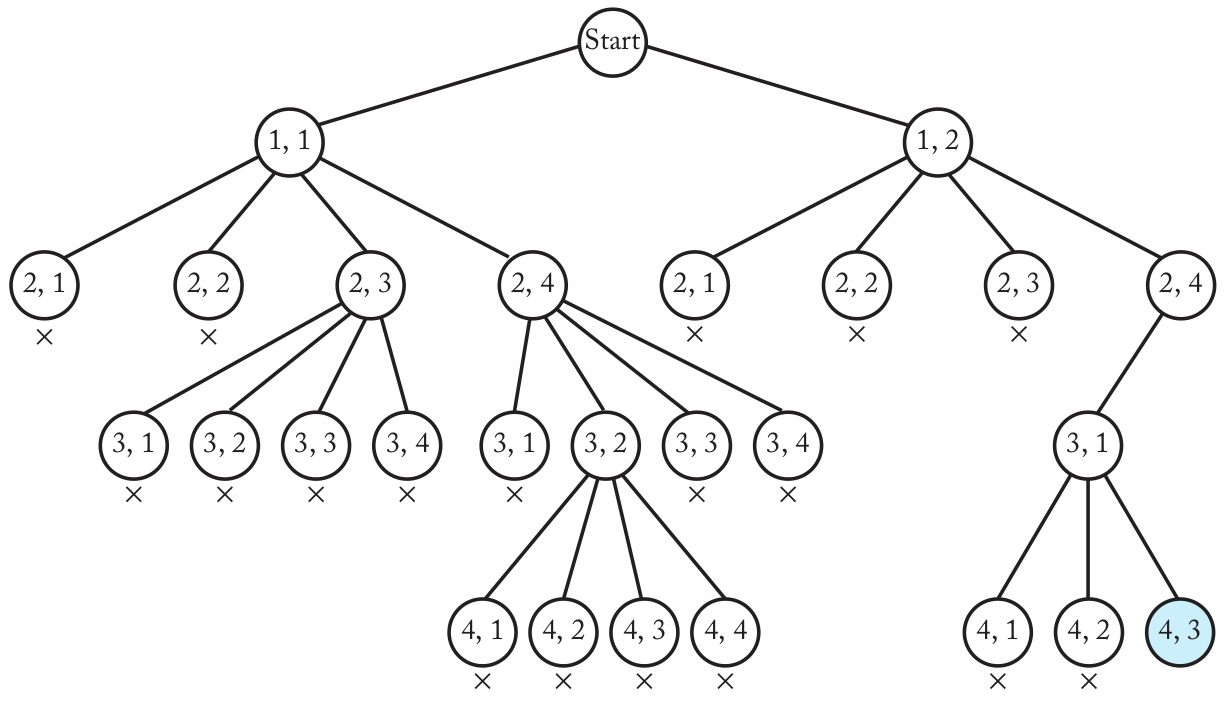
\includegraphics[width=0.7\textwidth]{figs/chap06/n-queens-tree2}
\end{figure}
\end{itemize}
\end{frame}


\begin{frame}{مسئلهٔ چند وزیر}
\begin{itemize}\itemr
\item[-]
در شکل زیر روند بررسی فضای حالت در صفحهٔ شطرنج نشان‌داده شده است.
\begin{figure}
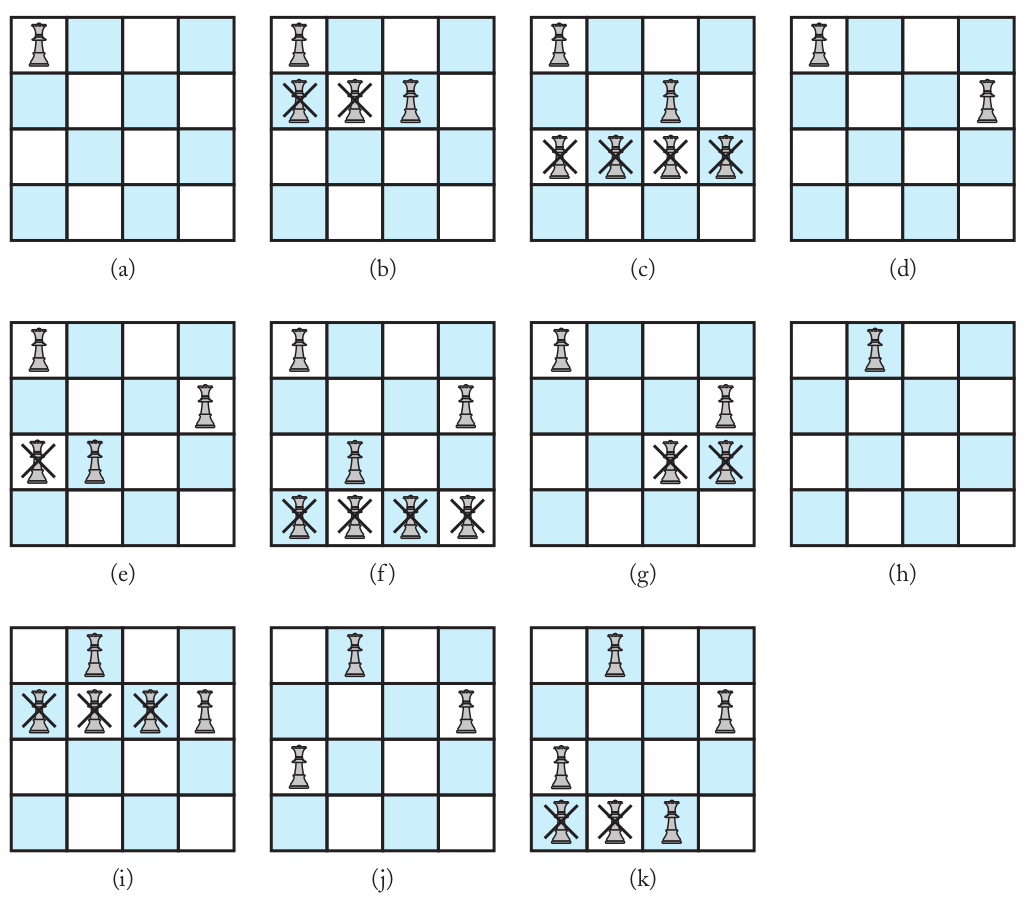
\includegraphics[width=0.5\textwidth]{figs/chap06/n-queens-board}
\end{figure}
\end{itemize}
\end{frame}


\begin{frame}{مسئلهٔ چند وزیر}
\begin{itemize}\itemr
\item[-]
تابع
promising
باید بررسی کند که آیا دو وزیر در یک ستون یا قطر قرار گرفته‌اند یا خیر.
\item[-]
اگر
\m{col(i)}
ستونی باشد که وزیر i ام در آن قرار گرفته است، باید بررسی کنیم که
\m{col(i)}
و
\m{col(j)}
برای هیچ دو وزیر i و j برابر نباشد.
\item[-]
همچنین دو وزیر به صورت مورب یکدیگر را تهدید می‌کنند اگر
\m{col(i) - col(j) = i - j}
و یا
\m{col(i) - col(j) = j - i}
باشد.
\end{itemize}
\end{frame}


\begin{frame}{مسئلهٔ چند وزیر}
\begin{itemize}\itemr
\item[-]
الگوریتم پسگرد برای مسئلهٔ چند وزیر به صورت زیر است. برای شروع الگوریتم تابع
\code{Queens(0)}
فراخوانی می‌شود.
\begin{algorithm}[H]\alglr
  \caption{Queens} 
  \begin{algorithmic}[1]
   \Func{Queens}{index i}
   \If{Promising(i)}
   		\If{i == n}
   				\State print col[1] through col[n]
   		\Else
   		\Statex \LeftComment{See if queen in (i+1)-st row can be}
   		\Statex \LeftComment{positioned in each of the n columns.}
   				\For{j = 1 \To n}
   					\State col[i + 1] = j
   					\State Queens(i + 1)	
   				\EndFor
   		\EndIf
  \EndIf                       
  \end{algorithmic}
  \label{alg:merge}
\end{algorithm}
\end{itemize}
\end{frame}


\begin{frame}{مسئلهٔ چند وزیر}
\begin{itemize}\itemr
\item[-]
\begin{algorithm}[H]\alglr
  \caption{Promising} 
  \begin{algorithmic}[1]
   \Func{Promising}{index i}
   \Statex  \LeftComment{Check if any queen k threatens queen in the i-th row.}	
   \For{k = 1 \To i - 1}	 
   			\If{col[i] == col[k] \textbf{or} |col[i] − col[k]| == i − k}
   					\State \Return false
   			\EndIf
   	\EndFor
   	\State \Return true                  
  \end{algorithmic}
  \label{alg:merge}
\end{algorithm}
\end{itemize}
\end{frame}


\begin{frame}{مسئلهٔ چند وزیر}
\begin{itemize}\itemr
\item[-]
حال می‌خواهیم الگوریتم پسگرد برای چند وزیر را تحلیل کنیم.
برای این کار تعداد رئوسی که در درخت فضای حالت بررسی می‌شوند را محاسبه می‌کنیم. از آنجایی که به دست آوردن تعداد دقیق حالات  وقتی حالت‌ها هرس می‌شوند ساده نیست، برای تعداد رئوس بررسی شده در درخت فضای حالت یک کران بالا در نظر می‌گیریم.
\item[-]
در درخت فضای حالات در سطح صفر، یک رأس داریم، در سطح یک تعداد n رأس، در سطح ۲ تعداد
\m{n^2}
رأس و در سطح n تعداد
\m{n^n}
رأس داریم. پس تعداد همهٔ رئوس بررسی شده برابر است با :
\begin{align*}
\m{1 + n + n^2 + n^3 + \cdots + n^n = \frac{n^{n+1} - 1}{n-1}}
\end{align*}
\item[-]
برای مسئله ۸ وزیر این تعداد برابر است با
\begin{align*}
\m{\frac{8^{8+1}-1}{8-1} = 19,173,961}
\end{align*}
\end{itemize}
\end{frame}


\begin{frame}{مسئلهٔ چند وزیر}
\begin{itemize}\itemr
\item[-]
حال یک کران بالای دیگر برای تعداد رئوس بررسی شده در نظر می‌گیریم. می‌دانیم که هیچ دو وزیری نمی‌توانند در یک ستون قرار بگیرند، بنابراین وقتی وزیر اول انتخاب شد، وزیر دوم تنها در ۷ مکان می‌تواند قرار بگیرد پس در سطح اول ۸ رأس و در سطح دوم
\LR{۸ $\times$ ۷}
رأس، در سطح سوم
\LR{۸ $\times$ ۷ $\times$ ۶}
رأس داریم و بدین ترتیب الی آخر.
\item[-]
پس در حالت کلی کران بالای رئوس بررسی شده برابراست با :
\begin{align*}
\m{1 + n + n(n-1) + n(n-1)(n-2) + \cdots + n!}
\end{align*}
\item[-]
برای مسئله ۸ وزیر این تعداد برابراست با
۱۰۹،۶۰۱
رأس.
\end{itemize}
\end{frame}


\begin{frame}{مسئلهٔ چند وزیر}
\begin{itemize}\itemr
\item[-]
تعداد دقیق رئوس بررسی شده را می‌توانیم با پیاده‌سازی الگوریتم به دست آوریم.
\item[-]
از آنجایی که کران بالای تعداد حالت مورد بررسی
\m{n!}
است، زمان اجرای الگوریتم پسگرد برای مسئلهٔ n وزیر
\m{O(n!)}
است.
\end{itemize}
\end{frame}
\iffalse
\begin{frame}{شاخه و کران}
\begin{itemize}\itemr
\item[-]
روش شاخه و کران
\fn{1}{branch and bound}
برای بهبود الگوریتم‌های پسگرد به کار می‌روند.
\item[-]
روش شاخه و کران، همچون روش پسگرد درخت فضای حالت را برای یافتن جواب بررسی می‌کند.
\item[-]
یک الگوریتم شاخه و کران در هر رأس درخت جستجوی حالات،
کرانی را محاسبه می‌کند که با استفاده از مقدار کران می‌توان گفت آیا آن رأس
 امید دهنده است یا خیر. مقداری که به عنوان کران در هر رأس محاسبه می‌شود، با استفاده از کرانی بر روی جواب مسئله به دست می‌آید.
\end{itemize}
\end{frame}
\fi

\begin{frame}{شاخه و کران}
\begin{itemize}\itemr
\item[-]
روش شاخه و کران
\fn{1}{branch and bound}
 همچون روش پسگرد درخت فضای حالت را برای یافتن جواب بررسی می‌کند.
\item[-]
این روش معمولاً برای مسائل بهینه‌سازی استفاده می‌شود. در مسائل بهینه‌سازی هدف یافتن جواب بهینه (کوچکترین، بزرگترین، ...) است. در هر لحظه در هنگام پیمایش درخت فضای حالت یکی از جواب‌های به دست آمده تا آن لحظه بهینه است. بنابراین قبل از بسط دادن یک رأس می‌توانیم محاسبه کنیم آیا جوابی که با بسط دادن آن رأس به دست می‌آید، از جواب بهینه‌ای که تا آن لحظه به دست آمده است، بهتر است یا خیر. در صورتی که امیدی به یافتن جواب بهتر نبود، رأس مورد پیمایش بسط داده نمی‌شود.
\item[-]
بنابراین اگر با بسط دادن یک رأس امید به یافتن جواب بهینه‌تر وجود نداشت، می‌گوییم آن رأس نومیدکننده
\fn{2}{nonpromising}
است، در غیر اینصورت امیددهنده
\fn{3}{promising}
است.
یک الگوریتم شاخه و کران در هر رأس درخت جستجوی حالات،
کرانی را محاسبه می‌کند که با استفاده از مقدار کران می‌توان گفت آیا آن رأس
 امید دهنده است یا خیر.
\end{itemize}
\end{frame}


\begin{frame}{شاخه و کران}
\begin{itemize}\itemr
\item[-]
می‌توانیم مسئلهٔ کوله پشتی ۱-۰ را با استفاده از روش پسگرد حل کنیم.
\item[-]
در سطح اول در درخت فضای حالت، دو حالت بررسی می‌شوند : (۱) کالای اول در کوله پشتی قرار می‌گیرد، یا (۲) کالای اول در کوله‌پشتی قرار نمی‌گیرد. همینطور در سطح دوم به ازای هر یک از دو حالت سطح اول درخت، باید دو حالت بررسی شوند : اینکه کالای دوم در کوله‌پشتی قرار می‌گیرد یا نمی‌گیرد.
این فرایند ادامه پیدا می‌کند تا به یک جواب برسیم و هزینه کوله‌پشتی را محاسبه کنیم. در یک الگوریتم پسگرد باید همهٔ برگ‌های درخت فضای حالت بررسی شده، برگی که بیشترین هزینه را دارد انتخاب شود. 
\end{itemize}
\end{frame}

\begin{frame}{شاخه و کران}
\begin{itemize}\itemr
\item[-]
همچنین در حل این مسئله
 می‌توان از روش شاخه و کران استفاده کرد. برای بررسی اینکه
 یک رأس امیددهنده است یا خیر،
باید محاسبه کنیم که آیا حداکثر ارزشی که می‌تواند با برداشتن باقی اشیاء حاصل شود، از جواب بهینهٔ به دست آمده تا آن لحظه بیشتر است یا خیر.
تنها در صورتی بسط یک رأس را ادامه می‌دهیم که امیدی به بهبود جواب داشته باشیم.
\item[-]
یک الگوریتم شاخه و کران به ازای هر رأس در درخت فضای حالت محاسبه می‌کند آیا هزینه‌ای که با بسط آن رأس به دست می‌آید از جواب بهینه به دست آمده بهتر خواهد بود یا خیر. به عبارت دیگر می‌گوییم در هر رأس یک کران محاسبه می‌شود و با استفاده از کران محاسبه شده تصمیم گرفته می‌شود رأس مورد بررسی هرس شود یا خیر.
%\item[-]
%در هر لحظه در حین اجرای الگوریتم پسگرد، یکی از جواب های به دست آمده جواب بهینه است. در هر رأس درخت فضای حالت برای اجناس باقیمانده خارج از کوله پشتی یک کران بالا با استفاده از الگوریتم حریصانه (با فرض این که اجناس را می‌توان تقسیم کرد) به دست می‌آوریم. اگر مقدار این کران بالا از جواب بهینه به دست آمده تا آن لحظه کمتر بود، آن رأس را بسط نمی‌دهیم زیرا امیدی به پیدا کردن جواب بهینه با بسط آن رأس وجود نخواهد داشت.
\end{itemize}
\end{frame}

\begin{frame}{شاخه و کران}
\begin{itemize}\itemr
\item[-]
در روش شاخه و کران، با استفاده از مقدار کران به دست آمده، نه تنها می‌توان تصمیم گرفت که یک رأس بسط داده شود و یا خیر، بلکه می‌توان علاوه بر آن با استفاده از کران به دست آمده، تصمیم گرفت کدام رأس برای بسط دادن مناسب‌تر است.
\item[-]
با استفاده از این روش معمولاً می‌توان با سرعت بیشتری به جواب بهینه دست پیدا کرد.
\item[-]
به این روش جستجوی بهتر اول
\fn{1}{best-first search}
با هرس کردن شاخه و کران
\fn{2}{branch and bound pruning}
گفته می‌شود.
\end{itemize}
\end{frame}


\begin{frame}{شاخه و کران}
\begin{itemize}\itemr
\item[-]
در جستجوی بهتر اول، درخت فضای حالت را با استفاده از جستجوی سطح اول
\fn{1}{breadth-first search}
 پیمایش می‌کنیم.
%در جستجوی درخت فضای حالت گاهی به جای جستجوی عمق اول، از جستجوی سطح اول
%\fn{1}{breadth-first search}
%استفاده می‌شود.
\item[-]
در پیمایش سطح اول، ابتدا ریشه بررسی می‌شود، سپس رئوس سطح یک و پس از آن رئوس سطح دو و بدین ترتیب همهٔ رئوس تا برگ‌ها بررسی می‌شوند.
\item[-]
برخلاف جستجوی عمق اول که در آن از یک الگوریتم بازگشتی استفاده می‌شود، در جستجوی سطح-اول از یک صف برای پیمایش رئوس درخت استفاده می‌کنیم.
\item[-]
بدین ترتیب فرزندان یک رأس در صف قرار می‌گیرند و به ترتیب فرزندان یک به یک از صف خارج شده و فرزندانشان پیمایش می‌شوند. بنابراین در این روش ابتدا سطح اول درخت، سپس سطح دوم و به همین ترتیب همهٔ سطوح پیمایش می‌شوند. به همین دلیل به این جستجو سطح-اول گفته می‌شود.
\end{itemize}
\end{frame}


\begin{frame}{شاخه و کران}
\begin{itemize}\itemr
\item[-]
الگوریتم زیر الگوریتم جستجوی درخت با استفاده از روش سطح-اول را نشان می‌دهد.
\begin{algorithm}[H]\alglr
  \caption{Breadth-First-Tree-Search} 
  \begin{algorithmic}[1]
   \Func{Breadth-First-Tree-Search}{tree T}
   \State queue Q
   \State node u, v
   \State initialize(Q)		\LeftComment{initialize Q to be empty.}
   \State u = root(T)
   \State visit(u)
   \State enqueue(Q, u)
   \While{!empty(Q)}
   		\State v = dequeue(Q)
   		\For{each child u of v}
   				\State visit(u)
   				\State enqueue(Q, u)
   		\EndFor
   \EndWhile                        
  \end{algorithmic}
  \label{alg:merge}
\end{algorithm}
\end{itemize}
\end{frame}

\begin{frame}{مسئلهٔ فروشندهٔ دوره‌گرد}
\begin{itemize}\itemr
\item[-]
یک فروشندهٔ دوره‌گرد می‌خواهد برای فروش اجناس خود به همهٔ شهرها سفر کند.
هر دو شهر می‌توانند توسط یک جادهٔ یک طرفه به یکدیگر متصل شده باشند و هر جاده طولی معین دارد.
فروشندهٔ دوره‌گرد می‌خواهد از شهر خود سفر را آغاز کند و مسیری را بپیماید که از هر شهر تنها یک بار عبور کند و در پایان به شهر خود بازگردد.
در ضمن می‌خواهد مسیر پیموده شده کوتاهترین مسیر باشد.
\item[-]
این مسئله را با استفاده از یک گراف مدلسازی می‌کنیم.
در یک گراف جهت‌دار، می‌خواهیم کوتاه‌ترین مسیری را پیدا کنیم که از یک رأس آغاز می‌شود، از هریک از رئوس تنها یک بار عبور می‌کند و به رأس اول باز می‌گردد. چنین مسیری یک مسیر بهینه است. از آنجایی که این مسیر بهینه از همهٔ رئوس عبور می‌کند، بنابراین می‌توانیم از هر رأسی مسیر را آغاز کنیم. به مسیری که از هر رأس تنها یک بار عبور می‌کند مسیر همیلتونی می‌گوییم و به مسیری که از هر رأس تنها یک بار عبور کند و به رأس اول بازگردد یک دور همیلتونی می‌گویند. در اینجا به دنبال کوتاهترین دور همیلتونی می‌گردیم.
\end{itemize}
\end{frame}


\begin{frame}{مسئلهٔ فروشندهٔ دوره‌گرد}
\begin{itemize}\itemr
\item[-]
در شکل زیر ماتریس مجاورت برای یک گراف جهت‌دار نشان داده شده است که در آن از هر رأس به رأس دیگر یک یال وجود دارد. اعداد در ماتریس مجاورت طول یال‌ها از یک رأس به رأس دیگرند. کوتاهترین دور همیلتونی در این گراف نشان داده شده است.
\begin{figure}
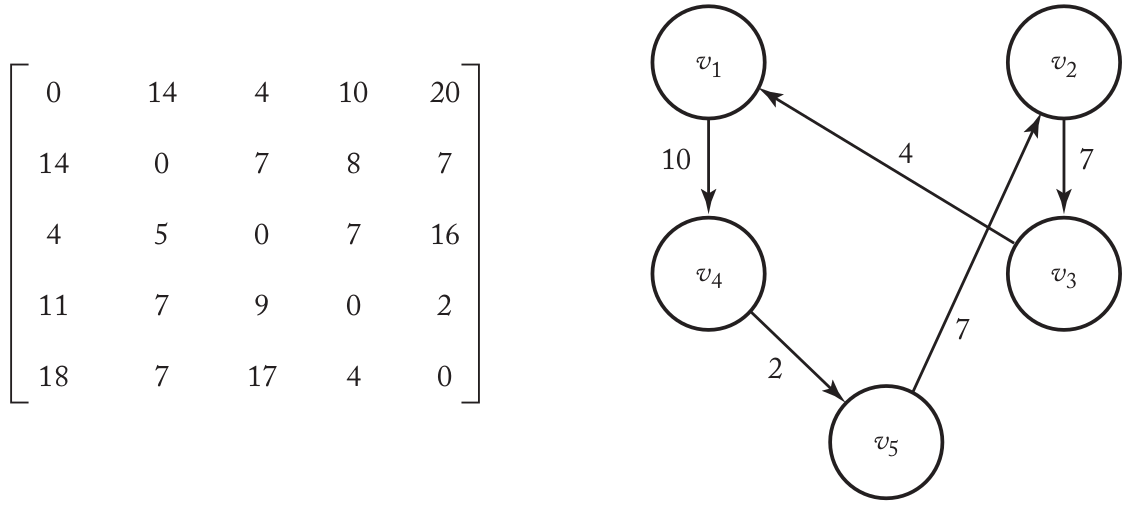
\includegraphics[width=0.7\textwidth]{figs/chap06/263-tsp}
\end{figure}
\end{itemize}
\end{frame}


\begin{frame}{مسئلهٔ فروشندهٔ دوره‌گرد}
\begin{itemize}\itemr
\item[-]
قسمتی از درخت جستجوی فضای حالت برای این مسئله در زیر نشان داده شده است.
\begin{figure}
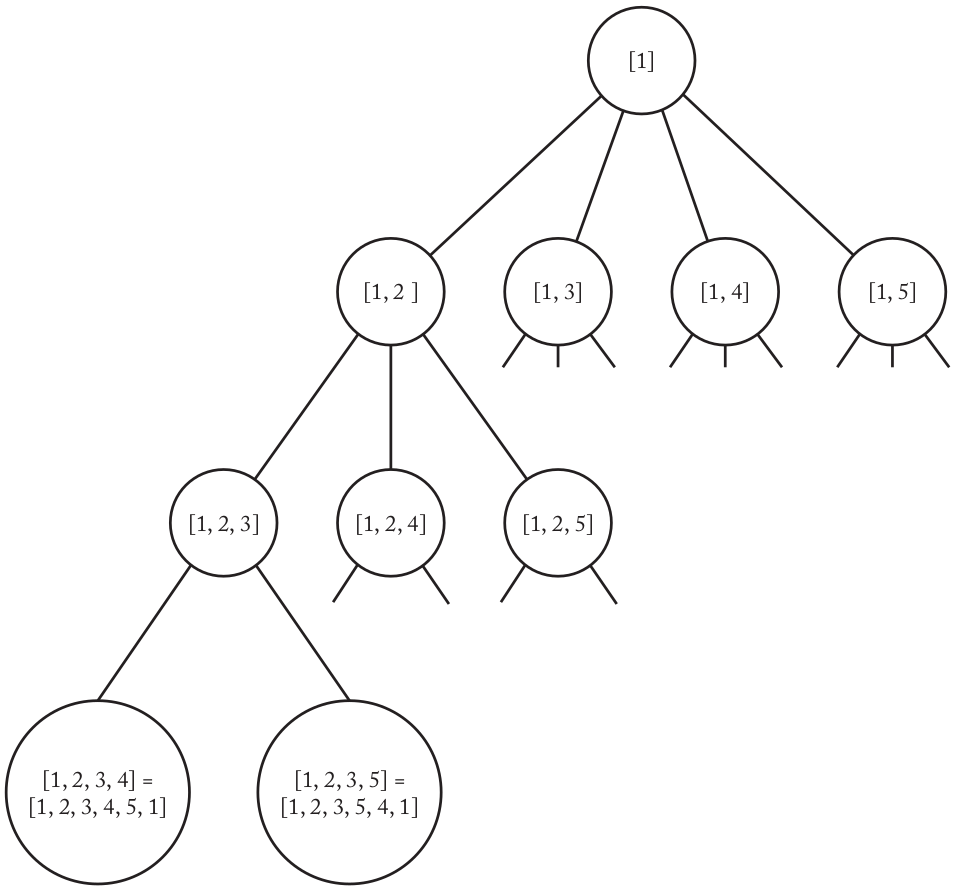
\includegraphics[width=0.5\textwidth]{figs/chap06/264-tsp}
\end{figure}
\end{itemize}
\end{frame}


\begin{frame}{مسئلهٔ فروشندهٔ دوره‌گرد}
\begin{itemize}\itemr
\item[-]
در این درخت فضای حالت، با رأس شماره ۱ از گراف آغاز می‌کنیم. مسیر بهینه ممکن است از هر یک از رئوس ۲ ، ۳ ، ۴ و ۵ عبور کند، بنابراین به ازای هریک از این رئوس یک فرزند در سطح یک در درخت فضای حالت می‌سازیم. رأس
\m{[1,2]}
در درخت فضای حالت مسیری را در گراف مشخص می‌کند که از رأس ۱ و ۲ در گراف عبور کند.
\end{itemize}
\end{frame}


\begin{frame}{مسئلهٔ فروشندهٔ دوره‌گرد}
\begin{itemize}\itemr
\item[-]
اکنون باید برای هر رأس در درخت فضای حالت یک مقدار کران پیدا کنیم. در هر رأس درخت فضای حالت یک کران پایین برای طول مسیری که می‌توان با بسط دادن آن رأس به دست آورد محاسبه می‌کنیم.
\item[-]
اگر کران پایین محاسبه شده در یک رأس از کوتاهترین مسیر همیلتونی به دست آمده تا آن لحظه کمتر باشد، آن رأس درخت فضای حالت امیددهنده است و آن رأس را بسط می‌دهیم، در غیر اینصورت آن رأس نومیدکننده است و بسط دادن را از آن رأس ادامه نمی‌دهیم.
\end{itemize}
\end{frame}


\begin{frame}{مسئلهٔ فروشندهٔ دوره‌گرد}
\begin{itemize}\itemr
\item[-]
برای محاسبهٔ کران به صورت زیر عمل می‌کنیم.
\item[-]
در هر رأس درخت فضای حالت تعدادی از رئوس گراف پیمایش شده و تعدادی پیمایش نشده‌اند.
به ازای رأس‌های پیمایش شده در گراف طول مسیر معین شده است. اما به ازای رأس‌های پیمایش نشده در گراف باید یک کران پایین برای طول مسیر محاسبه کنیم.
\item[-]
رأس پیمایش نشدهٔ
\m{V_i}
را در نظر بگیرید. جهت پیدا کردن یک کران پایین برای کوتاهترین مسیر،
به ازای هریک از رأس‌های پیمایش نشدهٔ
\m{V_i}
باید کوتاهترین یال خروجی از آن رأس را به صورت
\m{\min_{k} (V_i,V_k)}
 محاسبه کنیم و طول کوتاهترین یال‌های خروجی را به ازای همهٔ رئوس پیمایش نشده به صورت
\m{\sum_{i} \min_{k} (V_i,V_k)}
محاسبه کنیم.
\item[-]
 به عبارت دیگر به ازای هر یک از رئوس پیمایش نشدهٔ
\m{V_i}
باید یالی را پیدا کنیم که از
\m{V_i}
خارج می‌شود و کمترین هزینه را دارد.
مجموع طول این یال‌ها یک کران پایین برای طول مسیر است.
توجه کنید که این بدین معنا نیست که کوتاهترین‌ها الزاما در مسیر همیلتونی انتخاب می‌شوند، بلکه بدین معناست که هیچ مسیر همیلتونی با طول کمتر از مقدار محاسبه شده وجود نخواهد داشت.
\end{itemize}
\end{frame} 


\begin{frame}{مسئلهٔ فروشندهٔ دوره‌گرد}
\begin{itemize}\itemr
\item[-]
محاسبه کران را با یک مثال بررسی می‌کنیم. ماتریس مجاورت زیر را در نظر بگیرید.
\begin{figure}
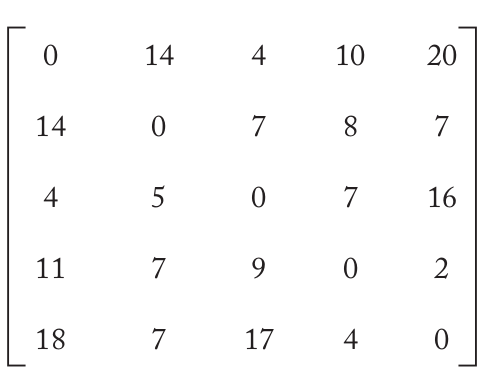
\includegraphics[width=0.2\textwidth]{figs/chap06/263-tsp-matrix}
\end{figure}
\item[-]
در ریشه درخت فضای حالت هیچ‌یک از رئوس گراف پیموده نشده‌اند. کران پایین مسیر در ریشه را می‌توانیم توسط رابطهٔ
\m{\sum_i \min_k (V_i,V_k)}
محاسبه کنیم. این مقدار برابراست با :
\begin{align*}
\m{\sum_i \min_k (V_i,V_k) = 4 + 7 + 4 + 2 + 4 = 21}
\end{align*}
\item[-]
بنابراین طول کوتاه‌ترین مسیر ممکن با شروع از رأس 
\m{V_1}
برابر است با ۲۱ .
\end{itemize}
\end{frame} 

\begin{frame}{مسئلهٔ فروشندهٔ دوره‌گرد}
\begin{itemize}\itemr
\item[-]
حال به ازای همهٔ فرزندان ریشه یک کران محاسبه می‌کنیم.
%و رأسی را برای پیمایش انتخاب می‌کنیم که کران محاسبه شده برای آن کمینه باشد.
برای مثال
 رأس
\m{[1,2]}
در درخت فضای حالت را در نظر بگیرید. یالی با طول
\m{14}
از رأس
\m{V_1}
به رأس
\m{V_2}
پیموده شده است.
طول کوتاهترین مسیری که با ادامهٔ این مسیر می‌تواند وجود داشته باشد برابر خواهد بود با ۱۴ به علاوه کوتاهترین مسیری که از بقیه رئوس به غیر از 
\m{V_2}
 عبور می‌کند. توجه کنید که از آخرین رأس در مسیر که در اینجا
\m{V_2}
است،
نمی‌توانیم به اولین رأس در مسیر که در اینجا
\m{V_1}
است،
بازگردیم اما امکان این که از هر یک از رئوس دیگر به 
\m{V_1}
برویم وجود دارد.
\begin{figure}
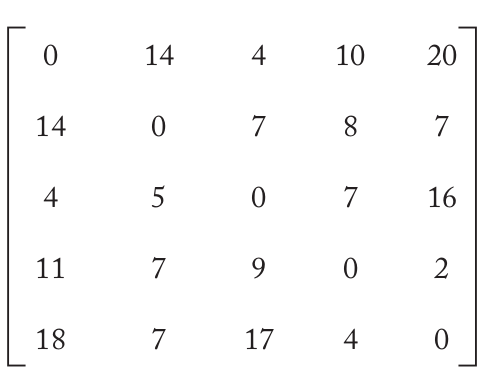
\includegraphics[width=0.2\textwidth]{figs/chap06/263-tsp-matrix}
\end{figure}
\item[-]
 کران پایین مسیر در این رأس برابراست با :
\begin{align*}
\m{14 + \sum_{i\in \{2,3,4,5 \}} min_k(V_i,V_k) = 14 + 7 + 4 + 2 + 4 = 31}
\end{align*}
\end{itemize}
\end{frame} 


\begin{frame}{مسئلهٔ فروشندهٔ دوره‌گرد}
\begin{itemize}\itemr
\item[-]
بدین ترتیب می‌توانیم مقدار کران را در هر‌یک از رئوس درخت فضای حالت به صورت زیر محاسبه کنیم.
\begin{figure}
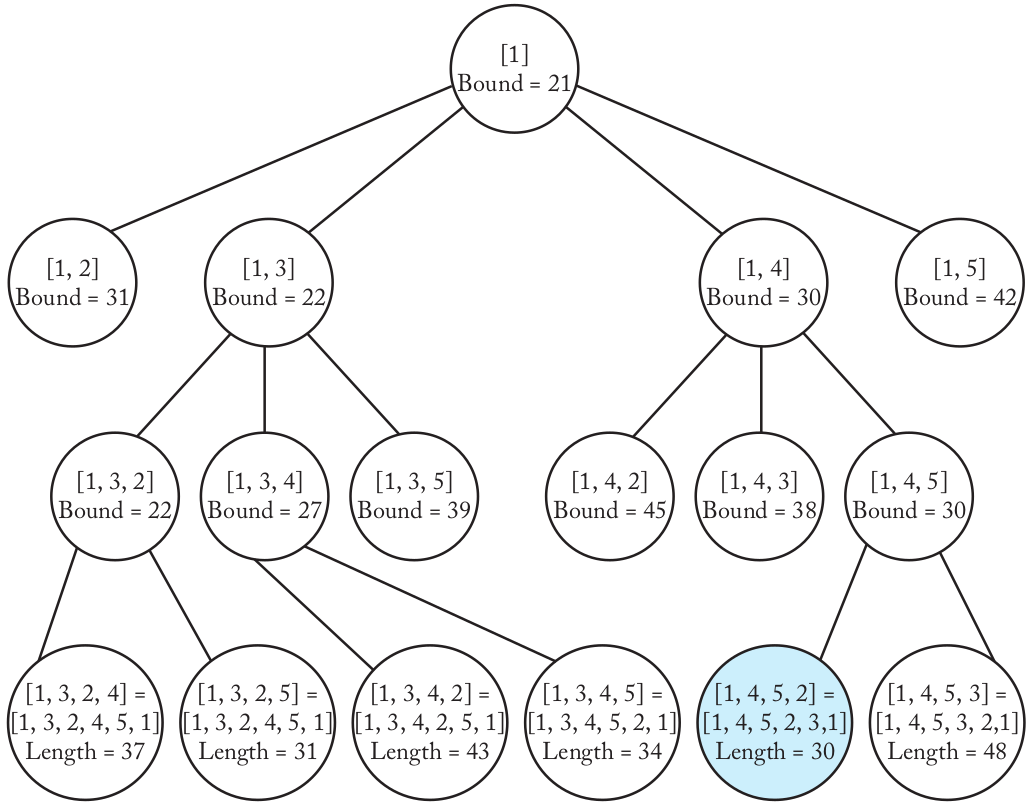
\includegraphics[width=0.5\textwidth]{figs/chap06/267-tree}
\end{figure}
\end{itemize}
\end{frame} 


\begin{frame}{مسئلهٔ فروشندهٔ دوره‌گرد}
\begin{itemize}\itemr
\item[-]
مقدار کران را برای همهٔ رئوس محاسبه می‌کنیم و رأسی را برای بسط دادن انتخاب می‌کنیم که مقدار کران آن کمینه باشد.
\item[-]
در اینجا از بین رئوس
\m{[1,2], [1,3], [1,4], [1,5]}
رأس 
\m{[1,3]}
کوچکترین کران را دارد که برابر با ۲۲ است.
\item[-]
وقتی رأس 
\m{[1,3]}
بسط داده شد، در نهایت کوتاهترین طول مسیری که در ریشه به دست می‌آید برابر با ۳۱ است.
\item[-]
اما در رأس 
\m{[1,4]}
همچنان یک کران کوچکتر برابر با ۳۰ وجود دارد،‌ بنابراین آن رأس را بسط می‌دهیم و در نهایت مسیری با طول ۳۰ پیدا می‌کنیم.
\end{itemize}
\end{frame} 


\begin{frame}{مسئلهٔ فروشندهٔ دوره‌گرد}
\begin{itemize}\itemr
\item[-]
هر رأس در درخت فضای حالت را می‌توانیم با ساختمان زیر نشان دهیم.
\begin{algorithm}[H]\alglr
\caption{Node Structure} 
\begin{algorithmic}[1]
\Statex \textbf{struct} node
\State~~ int level \LeftComment{the node’s level in the tree}
\State~~ ordered-set path
\State~~ int bound
\end{algorithmic}
\label{alg:node-structure}
\end{algorithm}
\end{itemize}
\end{frame} 


\begin{frame}{مسئلهٔ فروشندهٔ دوره‌گرد}
\begin{itemize}\itemr
\item[-]
در الگوریتم زیر برای یک گراف با n رأس، که وزن یال‌های آن با ماتریس W داده شده است، می‌خواهیم کوتاهترین دور همیلتونی را پیدا کنیم.
\begin{algorithm}[H]\alglr
  \caption{Travelling Salesman Problem} 
  \begin{algorithmic}[1]
   \Func{Travelling-Salesman-Problem}{int n, int-matrix W}
   \State ordered-set opttour \LeftComment{Optimal tour}
   \State int minlength = $\infty$ \LeftComment{The length of the optimal tour}
   \State priority-queue PQ
   \State node v
   \State initialize(PQ)		\LeftComment{Initialize PQ to be empty.}
   \State v.level = 0
   \State v.path = [1]	\LeftComment{Make first vertex the}
   \State v.bound = bound(v)		\LeftComment{starting one.}
   \State insert(PQ,v)                           
  \end{algorithmic}
  \label{alg:tsp1}
\end{algorithm}
\end{itemize}
\end{frame} 


\begin{frame}{مسئلهٔ فروشندهٔ دوره‌گرد}
\begin{center}
\resizebox{.74\textwidth}{!}{
\begin{minipage}{\textwidth}
\begin{algorithm}[H]\alglr
  \caption{Travelling Salesman Problem} 
  \begin{algorithmic}[1]
  \setcounter{ALG@line}{9}
  % \Func{Travel2}{int n, const number W[] [], ordered-set\& opttour, number\& minlength}
   \While{!empty(PQ)}
   	  \State remove(PQ, v)\LeftComment{Remove node with best bound.}
   	  \If{(v.bound < minlength)}
   			   \For{(all i not in v.path)}
   			           %\State create new node u
   			           \State create the new tree node u
   			           \State u.level = v.level + 1\LeftComment{Set u to a child of v.}
   					   \State u.path = [v.path , i] \LeftComment{put i at the end of v.path}
						\Statex \LeftComment{Check if next vertex completes a tour.}   					   
   					   \If{(u.level == n-2)}
							\Statex \LeftComment{put the last vertex not in u.path and also vertex 1 at the end of u.path}   					       
   					        \State u.path = [u.path, last-vertex, 1]
                           \Statex \LeftComment{Function length computes the length of the tour.}   							
   							\If{(length(u) < minlength)}
   									\State minlength = length(u)
   									\State opttour = u.path
   							\EndIf
   					   \Else
   							\State u.bound = bound(u)
   					        \If{(u.bound < minlength)}
   							   \State insert(PQ, u)
   					         \EndIf
   					   \EndIf
   		   \EndFor
   	   \EndIf
   \EndWhile     
   \State \Return (opttour, minlength)                         
  \end{algorithmic}
  \label{alg:tsp2}
\end{algorithm}
\end{minipage}
}
\end{center}
\end{frame}



\begin{frame}{مسئلهٔ فروشندهٔ دوره‌گرد}
\begin{itemize}\itemr
\item[-]
کران یک رأس درخت فضای حالت را به صورت زیر محاسبه می‌کنیم.
\begin{center}
\resizebox{.8\textwidth}{!}{
\begin{minipage}{\textwidth}
\begin{algorithm}[H]\alglr
\caption{Computing Bound for Travelling Salesman Problem} 
  \begin{algorithmic}[1]
   \Func{bound}{node v}
   \State bound = 0  
   \For{edge (i,j) in v.path}
       \State bound += length(i,j)
   \EndFor  
   %\State min = $\infty$
   \State i = last vertex in v.path
   \State min = $\min_k$ \{ W[i][k], vertex k $\not\in$ v.path \}
   %\For{vertex k not in v.path}
   %        \If{W[i][k] < min}
   %            \State min = W[i][k]
   %        \EndIf
   %    \EndFor  
   \State bound += min      
   \For{vertex i $\not\in$ v.path}
   \State min = $\min_k$ \{ W[i][k], vertex k $\not\in$ v.path \textbf{or} k = 1 \}
       %\State min = W[i][1]
       %\For{vertex k not in v.path}
       %    \If{W[i][k] < min}
       %        \State min = W[i][k]
       %    \EndIf
       %\EndFor
       \State bound += min
  \EndFor
  \State \Return bound
  \end{algorithmic}
  \label{alg:tsp-bound}
\end{algorithm}
\end{minipage}
}
\end{center}
\end{itemize}
\end{frame} 

\iffalse
\begin{frame}{مسئلهٔ فروشندهٔ دوره‌گرد}
\begin{itemize}\itemr
\item[-]
ممکن است در یک الگوریتم شاخه و کران بتوانیم چندین تابع کران پیدا کنیم که در این موارد معمولاً یکی از توابع، کران بهتری پیدا می‌کند.
\end{itemize}
\end{frame}
\fi

%%%%%%%%%%%%

%%%%%%%%%%%%
%\section*{References}
%\begin{frame}<0>[noframenumbering]
%\bibliographystyle{apalike}
%\bibliography{docs/bib}
%\end{frame}
%%%%%%%%%%%%

\end{document}
